% !TEX root = Eco-Model.tex
\section{Design of the ecosystem} % (fold)
\label{sec:design_of_the_ecosystem}
\subsection{Preliminaries} % (fold)
\label{sub:preliminaries}
The manufacturing ecosystem we proposed in this paper consists of the structure of cloud manufacturing, the operation mode and the controlling rules. Before the detailed interpretation for these parts, we describe some basic settings as follows.

\subsubsection{Master plan} % (fold)
\label{ssub:master_plam}
With the cloud manufacturing platform operating, demander comes, signs up and publish orders. Match module in platform informs the task messages in the order to every matched resources and services. After the select decision makes by the demander, the selected resources and services prepare to the performance of the task. 
Providers find frequent task after a bunch of successful accomplishment via resource reviews, then another type of job, service-call generated by them to gather certain type and amount of resources registered in the platform to create service in order to perform the certain task more efficient than before. Most of resource related decision making are well controlled by platform with the review module.

A single order($o_i$) consists of a set $\mathcal{T}_i = \left\{ t_{i1},t_{i2},\dots,t_{in}\right\}$ of tasks which have to be processed. The tasks are interrelated by kinds of constraints. First, precedence constraints force task $t_{ij}$ not to be started before all its immediate predecessors, how to construct the predecessor will be explained later. Second, performing the tasks requires resources with limited capacities. Third, resources cooperation transmits and enhances these constraints.

A single resource($r_k$) belongs to one type in set $\mathcal{A} = \left\{1,2,\dots\,A\right\}$ given by the platform. While being processed via resource cooperation, task $t_{ij}$ requires $q_{k,ij}$ units amount of the resources with every type in $\mathcal{A}_{ij}\subset\mathcal{A}$ during every period of its non-preemptable duration $p_{ij}$. Each resource $r_k$ has a limited capacity of $C_k$ at any point in time.

A single service($s_l$) is a composition of all resources in set $R_l$ with their partial capacities, it can only process certain task with matched resource configuration($\mathcal{A}_{ij}=\mathcal{A}_l$,$Q_{k,ij}=Q_l$) without resource coordinating any more. While being processed via one matched service, task can be suspended then outsourced to other matched service or resource cooperation.
Resource comes along with provider when it enter the ecosystem, however, service doesn't, service is generated after a period of time, the prototype of a service is another type of job, we call it the service-call.

A single service-call($sc_l$) comes out after the finish of one frequent task, so it have the same resource configuration the frequent task. Service-call can only be performed via resource cooperation with duration $p_l$, because the identity of resource, the capacity cannot be return to the resource after the finish of service-call, so the service-call brings new constrains to the related resources. Unlike the task, the amount of one type resource required in the service-call can be pieced together from more than one resource as long as they are in the same type.

Specifically, a simple instance with configuration \autoref{tab:simplejobconfiguration}--\ref{tab:simpleresourceconfiguration} and schedule chart \autoref{fig:scheduleChart} will describe the setting more clearly. 
\begin{table}[htbp]
  \centering
  \scriptsize
  \caption{Simple job configuration}
    \begin{tabular}{cccccc}
    \toprule
    \multicolumn{1}{c}{\multirow{2}[0]{*}{ Job}} & \multicolumn{3}{c}{Need Resource Capacity} & \multicolumn{1}{c}{\multirow{2}[0]{*}{Release Time}} & \multicolumn{1}{c}{\multirow{2}[0]{*}{Duration}} \\
    \multicolumn{1}{c}{} & $Type_1$ & $Type_2$ & $Type_3$ & \multicolumn{1}{c}{} & \multicolumn{1}{c}{} \\
    \midrule
    $t_1$ & 0     & 5     & 7     & 0     & 7 \\
    $t_2$ & 7     & 5     & 7     & 4     & 5 \\
    $t_3$ & 6     & 0     & 5     & 2     & 3 \\
    $sc_1$ & 0     & 0     & 3    & 1     & 1 \\
    $sc_2$ & 2     & 7     & 6     & 3     & 1 \\
    \bottomrule
    \end{tabular}%
  \label{tab:simplejobconfiguration}%
\end{table}%
\begin{table}[htbp]
  \centering
  \scriptsize
  \caption{Simple resource configuration}
    \begin{tabular}{ccc}
    \toprule
    Resource & Type  & Capacity \\
    \midrule
    $r_1$ & 1     & 10 \\
    $r_2$ & 2     & 10 \\
    $r_3$ & 3     & 10 \\
    $r_4$ & 3     & 10 \\
    \bottomrule
    \end{tabular}%
  \label{tab:simpleresourceconfiguration}%
\end{table}%
\begin{figure}[htbp]
	\centering
	\resizebox{.8\textwidth}{!}{% !TEX root = flow_head.tex


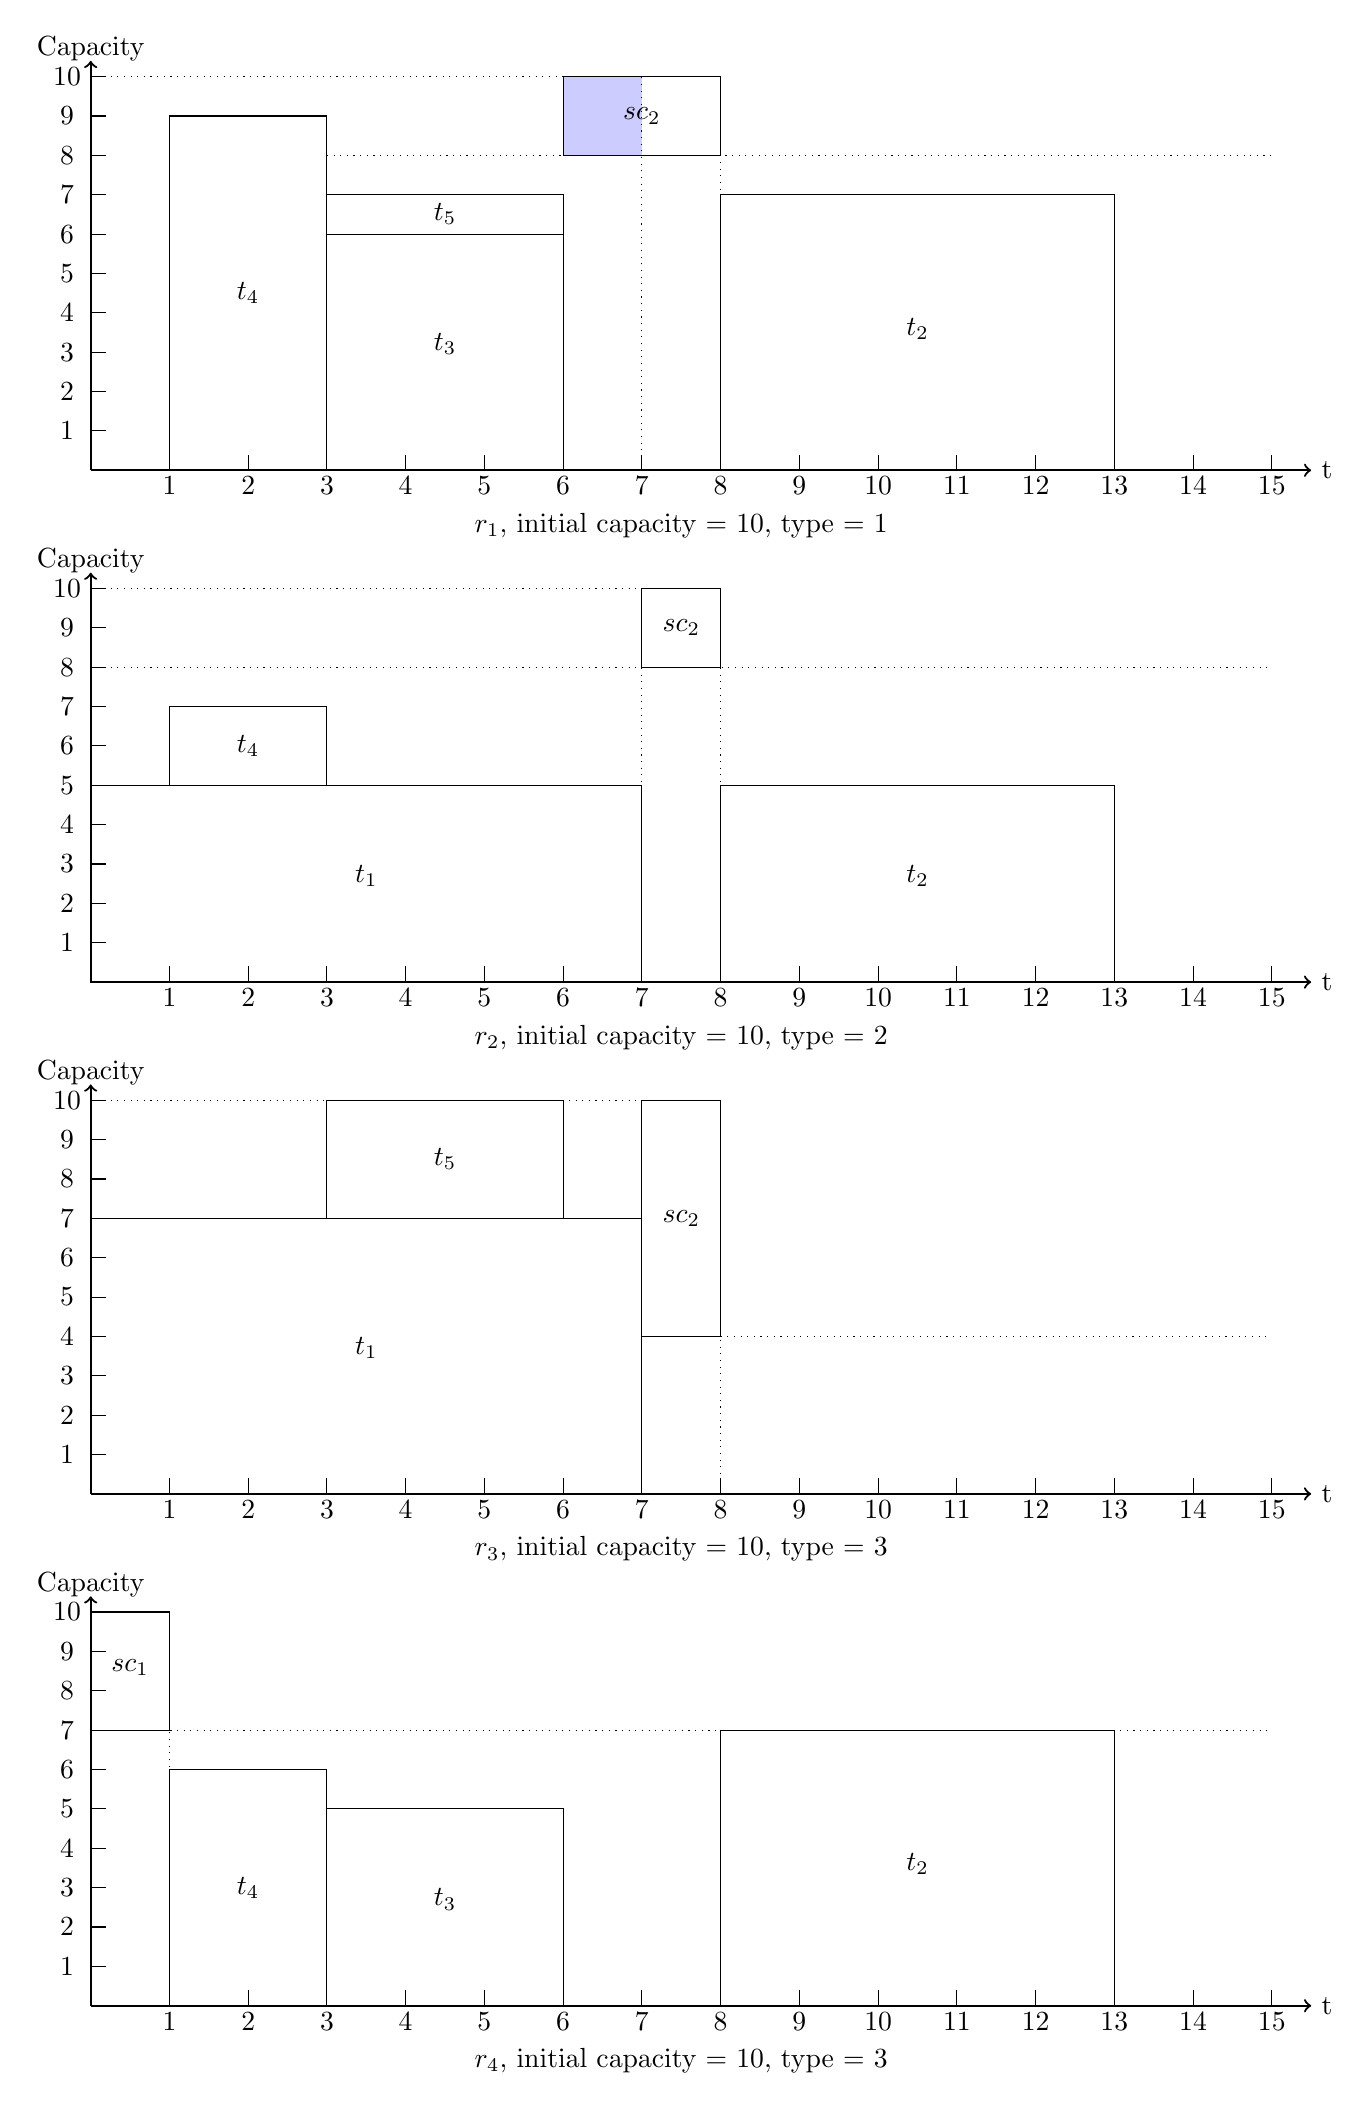
\begin{tikzpicture}
\foreach \x in {0,6.5,13,19.5}
	\draw [->,thick] (15.7cm,\x cm) node{t} (0,\x cm) -- +(15.5cm, 0) ;
\foreach \x in {0,6.5,13,19.5}
	\draw [->,thick] (0,\x cm) -- +(0,5.2 cm);
\foreach \x in {0,6.5,13,19.5}
	\draw[yshift=5.35cm] (0,\x cm) node{Capacity};
\foreach \x in {1,...,15}
	\foreach \y in {0,6.5,13,19.5}
		\draw (\x cm,\y cm) -- +(0,2mm);
\foreach \x in {1,...,15}
	\foreach \y in {0,6.5,13,19.5}
		\draw[yshift=-2mm] (\x cm,\y cm) node{$\x$};
\foreach \y in {0,6.5,13,19.5}
	\foreach \x in {1,...,10}
		\draw[yshift=\y cm] (0,0.5*\x cm) -- +(2mm,0) (-3mm,0.5*\x cm) node{$\x$};

\draw (7.5cm,-7mm) node{$r_4$, initial capacity = 10, type = 3};
\draw[yshift=6.5cm] (7.5cm,-7mm) node{$r_3$, initial capacity = 10, type = 3};
\draw[yshift=13cm] (7.5cm,-7mm) node{$r_2$, initial capacity = 10, type = 2};
\draw[yshift=19.5cm] (7.5cm,-7mm) node{$r_1$, initial capacity = 10, type = 1};

\fill[blue!20!,yshift=19.5cm] (6cm,4cm) rectangle (7cm,5cm);
\draw[yshift=19.5cm] (3cm,0) rectangle (6cm,3cm) (6cm,4cm) rectangle (8cm,5cm) (8cm,0) rectangle (13cm,3.5cm) (1cm,0) rectangle (3cm,4.5cm) (3cm,3cm) rectangle (6cm,3.5cm)  (4.5cm,1.6cm) node{$t_3$} (7cm,4.5cm) node{$sc_2$} (10.5cm,1.8cm) node{$t_2$} (2cm,2.25cm) node{$t_4$} (4.5cm,3.25cm) node{$t_5$};
\draw[dotted,yshift=19.5cm] (0,5cm) -- (7cm,5cm) (3cm,4cm) -- (15cm,4cm) (7cm,0) -- (7cm,5cm) (8cm,4cm) -- (8cm,3.5cm);
\draw[yshift=13cm] (0,0) rectangle (7cm,2.5cm) (7cm,4cm) rectangle (8cm,5cm) (8cm,0) rectangle (13cm,2.5cm) (1cm,2.5cm) rectangle (3cm,3.5cm)  (3.5cm,1.35cm) node{$t_1$} (7.5cm,4.5cm) node{$sc_2$} (10.5cm, 1.35cm) node{$t_2$}  (2cm,3cm) node{$t_4$};
\draw[dotted,yshift=13cm] (0,5cm) -- (7cm,5cm) (0,4cm) -- (15cm,4cm) (7cm,5cm) -- (7cm,0) (8cm,5cm) -- (8cm,0);
\draw[yshift=6.5cm] (0,0) rectangle (7cm,3.5cm) (7cm,2cm) rectangle (8cm,5cm) (3cm,3.5cm) rectangle (6cm,5cm) (3.5cm,1.85cm) node{$t_1$} (7.5cm,3.5cm) node{$sc_2$} (4.5cm,4.25cm) node{$t_5$};
\draw[dotted,yshift=6.5cm] (0,5cm) -- (7cm,5cm) (8cm,2cm) -- (15cm,2cm) (8cm,0) -- (8cm,2cm);
\draw (0,3.5cm) rectangle (1cm,5cm) (3cm,0) rectangle (6cm,2.5cm) (8cm,0) rectangle (13cm,3.5cm) (1cm,0) rectangle (3cm,3cm) (4.5cm, 1.35cm) node {$t_3$} (0.5cm,4.3cm) node{$sc_1$} (10.5cm,1.8cm) node{$t_2$} (2cm,1.5cm) node{$t_4$};
\draw[dotted] (0,3.5cm) -- (15cm,3.5cm) (1cm,0) -- (1cm,3.5cm);
\end{tikzpicture}
}
	\caption{Simple instance schedule chart}
	\label{fig:scheduleChart}
\end{figure}
This instance makes some simplification in the subscript fields in order to emphasize the resource cooperation, all the job(task and service-call) performance can only be started when the each of the related resource is ready, so the shadow in the figure is the waiting period. Horizontal dotted line constrained the available capacity of the resource for the following jobs, every performance of service-call will make the line lower and it will never get higher again unless the related service is repealed.

% subsubsection master_plan (end)

\subsubsection{Assumptions, nomenclature} % (fold)
\label{ssub:assumptions_nomenclature}
job
order
task
service-call
abstract machine
resource
service
demander
provider
platform
rank
hardness

detailed design will be explained in the following sections.
% subsubsection assumptions_nomenclature (end)
% subsection preliminaries (end)

\subsection{Operation mode} % (fold)
\label{sub:operation_mode}

% subsection operation_mode (end)

\subsection{Interactions and decisions} % (fold)
\label{sub:interactions_and_decisions}

% subsection interactions_and_decisions (end)

\subsection{Controlling rules} % (fold)
\label{sub:controlling_rules}

% subsection controlling_rules (end)

\subsection{Tricky problems} % (fold)
\label{sub:tricky_problems}
The job lock
% subsection tricky_problems (end)
% section design_of_the_ecosystem (end)